%%%%%%%%%%%%%%%%%%%%%%%%%%%%%%%%%%%%%%%%%%%%%%%%%%%%%%%%%%%%%%%%%%%%%%%%%%%%%%%%
\subsubsection{Grafické uživatelské rozhraní}

Pro prostředí LispWorks jsem k ExiLu implementoval minimalistické grafické
uživatelské rozhraní, zobrazené na obrázku \ref{gui} To sestává z hlavního okna
s deseti tlačítky organizovanými do tří řad (vpravo nahoře).

První řada tlačítek - \uv{Facts}, \uv{Templates}, \uv{Rules} a \uv{Agenda}
slouží k~zobrazení podoken s jednotlivými položkami. Okno \uv{Facts} zobrazuje
seznam faktů v pracovní paměti a umožňuje jejich odebrání tlačítkem
\uv{Retract fact}. Okno \uv{Templates} zobrazuje seznam definovaných šablon a
umožňuje jejich odebrání tlačítkem \uv{Undefine template}. Okno \uv{Rules}
zobrazuje seznam definovaných odvozovacích pravidel a umožňuje jejich odebrání
tlačítkem \uv{Undefine rule}. Poslední okno \uv{Agenda} zobrazuje seznam
aktuálních shod v agendě. Seznamy v~oknech se automaticky obnovují při každé
změně zobrazených hodnot.

Druhá řada tlačítek - \uv{Reset}, \uv{Step}, \uv{Run} a \uv{Halt} umožňuje
řízení inference. Tlačítka volají stejnojmenné funkce ExiLu.

Poslední řada tlačítek - \uv{Undo} a \uv{Redo} slouží k vracení a opětovnému
provedení akcí voláním stejnojmenných funkcí ExiLu.

\begin{figure}[h]
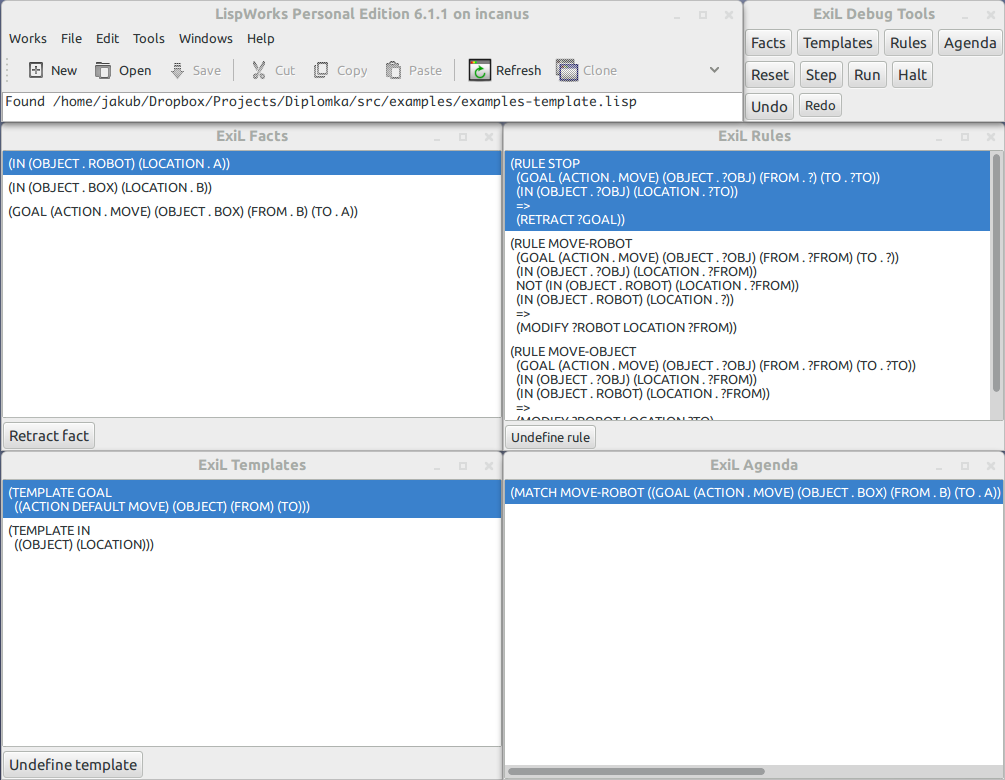
\includegraphics[width=\textwidth]{exil-gui.png}
\caption{Grafické uživatelské rozhraní}
\label{gui}
\end{figure}
